\chapter{Análise de dados}\label{chap:dese}

Neste capítulo será discutido o que foi feito nesta dissertação. Serão abordados requisitos para realizar o trabalho, as decisões tomadas e respetiva explicação e as dificuldades encontradas, que levaram a eventuais alterações aos objetivos inicialmente propostos. Serão ainda mostrados os vários tipos de análises efetuadas aos dados recolhidos, bem como alguns resultados daí obtidos. 

\section{Descrição do estudo}

Para que este estudo pudesse ser feito, o primeiro passo era ter um conjunto de dados de pacientes diabéticos de forma a ser analisado. Este conjunto de dados tinha que ter algumas características específicas para que pudesse ser utilizado da forma pretendida: tinha que ser um conjunto de registos para cada paciente ao longo de algum tempo, sendo que idealmente, no mínimo, cada paciente teria registos correspondentes a quatro semanas. Depois de uma pesquisa, foi possível concluir que não existia, na \textit{web}, qualquer \textit{data set} com estas características.
Para que este estudo pudesse ser feito, era necessário ter um \textit{data set} com os diferentes parâmetros que pudessem ser relevantes, como glicemia, insulina, hidratos de carbono e exercício. 
Como já mencionado, nenhum \textit{data set} existente \textit{on-line} tinha as características desejadas pois só possuíam um registo por pessoa e/ou o seu propósito era a classificação de um paciente como diabético ou não. O único \textit{data set} encontrado que tinha vários registos por pessoa ao longo do tempo tinha o inconveniente de ter apenas dados relativos a glicemias.

Face à falta de dados disponíveis, a solução encontrada foi recolher, de raíz, os dados para a criação do \textit{data set} desejável. Ao podermos construir o nosso próprio \textit{data set} tínhamos a vantagem de podermos recolher as variáveis que queríamos, e portanto, ter um conjunto de dados que torne este trabalho mais eficiente. Por outro lado, visto que a recolha dos dados seria feita através da aplicação MyDiabetes, havia a desvantagem desta ser ainda fechada ao público e, portanto, não ter doentes diabéticos a utilizá-la. Uma outra desvantagem era o tempo que a criação de um \textit{data set} com a variedade e tamanho desejáveis poderia levar. Por variedade e tamanho desejáveis entenda-se dados relativos a cerca de 20 pessoas durante algumas semanas.

Feitas as contas, apesar das desvantagens enunciadas, a solução seria mesmo recolher os dados através da aplicação, sendo que o primeiro passo seria arranjar voluntários. O processo de recolha de dados é descrito na próxima secção.

\section{Recolha de dados}

A recolha de dados foi feita em parceria com o Hospital de S. João, através do seu serviço de endocrinologia. Para tal, foi pedido à comissão de ética autorização para falar com os pacientes diabéticos do hospital e para que estes utilizassem a aplicação, enviando os respetivos registos, pedido esse que foi aceite. Qualquer paciente seria elegível para o projeto desde que tivesse mais de 18 anos e fosse insulino-dependente. 

O Dr. Celestino Neves, médico endocrinologista daquele serviço, serviu de ponte entre a faculdade e o hospital. Nesta primeira fase, o Dr. Celestino dava uma pequena explicação do projeto ao paciente antes, durante ou depois da consulta, sendo que depois re-encaminhava o paciente para nós, investigadores. Esta primeira abordagem do Dr. Celestino era bastante importante uma vez que tornava os pacientes mais recetivos à participação. No nosso encontro com os pacientes, explicávamos o que era o projeto, mostrando no que a aplicação consistia e como funcionava. Depois desta parte, dávamos a conhecer ao paciente os passos seguintes, nomeadamente a integração de um sistema de conselhos baseados no \textit{input} do utilizador. Durante este processo, explicávamos ao paciente a importância de termos dados reais de utilizadores e portanto a importância do envio dos registos, realçando que a longo prazo, os utilizadores seriam os maiores beneficiados, pois poderiam melhorar o seu controlo da glicemia. Os pacientes eram ainda informados que os registos enviados seriam utilizados apenas para fins de investigação e que, caso aceitassem participar no projeto, teriam de assinar um consentimento informado que explicava isso mesmo.

Se os pacientes aceitassem fazer parte do projeto, a aplicação era então instalada nos seus \textit{smartphones} e seria-lhes também dado acesso à aplicação na \textit{Google Play}. Assim, a aplicação passaria a estar sempre disponível para esse utilizador, mesmo que este formatasse ou trocasse o telemóvel, a partir da loja. Outra vantagem deste acesso seria os utilizadores poderem usufruir das atualizações entretanto feitas: sempre que houvesse uma atualização, apareceria o aviso e o utilizador poderia atualizar sem perder os registos já feitos.

Além da aplicação, eram também dadas aos voluntários as credenciais para terem acesso ao \textit{website} do projeto, para onde poderiam exportar os registos efetuados e visualizá-los através de gráficos. As credenciais garantiam assim que apenas os voluntários tinham acesso à parte privada da página, que tem tutoriais e a parte de visualização dos dados.


\subsection{Números e \textit{feedback}}

Este processo era feito duas vezes por semana, que correspondia aos dias de consultas da diabetes, durante aproximadamente três meses. Durante este tempo falámos com várias dezenas de pacientes, sendo que foi possível obter, logo à partida, uma conclusão: a esmagadora maioria dos pacientes com quem falámos estavam bastante recetivos à ideia e concordavam que podia ser uma mais-valia na melhoria da sua qualidade de vida. Muito poucos pacientes tinham a opinião de que a aplicação não teria utilidade, principalmente devido ao facto de estes utilizarem bomba, que torna o processo de controlo da glicemia muito mais reduzido e simples.
Além da idea em si, que foi bastante bem recebida, os utilizadores também deram \textit{feedback} positivo relativamente ao \textit{design} e funcionalidades da aplicação. 

Apesar de todos os pacientes acharem boa ideia ter uma aplicação como esta, nem todos se tornaram voluntários devido a diferentes razões: 1) nem todos os utilizadores tinham \textit{smartphone} e cerca de metade dos pacientes tinha outro sistema operativo que não Android e 2) alguns pacientes com idade mais avançada ou com outros problemas de saúde simplesmente não tinham tempo ou não disponibilidade para participar como voluntário. 
No final deste período tínhamos conseguido a participação de 31 voluntários. Apesar de este número ser suficiente para o que se pretendia, pois inicialmente tinha sido definido como objetivo pelo menos 20 participantes, nem todos os voluntários enviaram, de facto, os registos. 
Dos 31 voluntários apenas 8 enviaram registos pelo menos uma vez e apenas 5 destes enviaram registos relativamente a algumas semanas. Isto foi um dos principais problemas encontrados: para integrar um sistema de aconselhamento baseado nos dados introduzidos numa aplicação para \textit{smartphone} é fundamental saber que tipo de avisos ou conselhos se deve ou não mostrar. Por exemplo, um conselho como "Ajuste a insulina à quantidade de hidratos de carbono ingerida" é algo óbvio e que qualquer paciente diabético sabe, e portanto não seria uma grande mais valia para a alicação. Por outro lado, um aviso como "Hoje é segunda-feira e geralmente à segunda-feira tem valores de glicemia mais elevados" pode ser útil porque possivelmente é um padrão que o paciente não detetou. Neste caso, este conselho poderia fazer o utilizador controlar mais frequentemente a sua glicemia às segundas-feiras e, portanto, normalizar os valores das segundas-feiras a partir daí. 

Esta distinção entre avisos ou conselhos realmente úteis ou descartáveis é importante: se a aplicação mostrar demasiados conselhos intuitivos ou regras "banais" das quais os utilizadores já tenham conhecimento, estes podem acabar por achar que a aplicação não traz benefícios. Pelo contrário, se a aplicação mostrar conselhos baseados em comportamentos errados para cada utilizador, estes podem aperceber-se de que realmente têm esses comportamentos errados e usufruir verdadeiramente deste sistema de aconselhamento. 

Para fazer esta distinção torna-se importante obter a maior quantidade e variedade possível de dados. Imaginemos que temos apenas um \textit{data set} de um paciente com registos de uma semana. Esta quantidade de dados não permite concluir nada sobre eventuais regras descobertas nem sequer permite descobrir vários tipos de regras; tanto a variedade de pacientes como a quantidade de registos serão demasiado reduzidas para tal. 

Da mesma forma, os registos de 5 pacientes, embora seja obviamente mais vantajoso do que o registo de apenas 1 paciente, não é suficiente para esta parte. Uma vez mais, 5 pacientes não oferecem muita quantidade nem variedade em relação a rotinas ou comportamentos errados, que se traduz na variedade de regras produzidas. 

O objetivo da aplicação é gerar os tais conselhos de forma automática e, pensado desta forma, esta parte inicial pode parecer inútil: para quê estar a gerar regras se elas não vão ser utilizadas na aplicação em si? 

Esta questão prende-se, uma vez mais, com a filtragem de regras úteis ou não. Os registos de um único paciente podem gerar, por exemplo, centenas ou até milhares de regras. Obviamente que em milhares de regras muitas vão ser bastante parecidas e a esmagadora maioria vão ser regras que não têm relevância. É possível, por exemplo, que em alguns milhares de regras só se consiga aproveitar 5 ou 6. A importância de ter registos de vários pacientes prende-se com a variedade das regras geradas: dois pacientes podem gerar poucas regras cada um mas essas regras serem diferentes, ou seja, relativas a rotinas ou anomalias com efeitos ou causas diferentes. Esta análise dos dados à procura de regras servirá, então, para construir um conjunto de regras passíveis de ocorrer no dia-a-dia de um diabético que serão então integradas nesta aplicação. Assim, serão apenas detetados padrões e situações que possam ter alguma relevância e conselhos como "Adeque a insulina aos hidratos de carbono" não serão mostrados. Isto porque apesar de ser um bom conselho, também é óbvio e portanto provavelmente será tido como um conselho inútil por parte dos utilizadores. 

Ao ter esta filtragem para mostrar apenas conselhos realmente importantes, não só diminuiremos a quantidade de vezes que algum conselho é mostrado, tornando assim a aplicação menos "chata" para os utilizadores, como também tornam os conselhos mais especiais, ou seja, se um conselho ou aviso é mostrado é porque o utilizador tem de facto algum comportamento errado e que pode ser corrigido.

Neste sentido, a pouca quantidade de voluntários que enviaram registos foi a primeira dificuldade encontrada e que nos fez alterar a estratégia: uma vez que os dados existentes não seriam suficientes para fazer o sistema de aconselhamento de uma forma tão fidedigna quanto desejável, esse objetivo foi posto de lado. Face a estas novas circunstâncias, o objetivo passou a ser analisar os dados existentes das mais variadas formas para ver que tipo de conclusões se consegue obter. Os diferentes tipos de análises feitas vão ser descritos ainda neste capítulo.

Apesar de os dados serem poucos, a parte positiva é que estavam no formato pretendido e portanto o passo seguinte era começar a tratá-los.


\subsection{O \textit{data set}}

Os registos dos utilizadores são armazenados no telemóvel numa base de dados \textit{sqlite}[sqlite] que é depois convertida para um ficheiro csv através de um \textit{script}.[script] O \textit{script} converte cada uma das tabelas num ficheiro csv e depois, os ficheiros csv que interessa manter são copiados para um único ficheiro através do comando \textit{copy}.
 Os dados recebidos contêm alguns dados que são descartados, como os dados pessoais do utilizador, registo de peso ou medicação, que não são tão relevantes para a análise. Mesmo relativamente a algumas variáveis, como a glicemia por exemplo, só nos interessa saber o valor e a hora, e portanto todos os outros dados sobre a glicemia são apagados, como o "ID", "Tag" que é um valor opcional que pode associar a medição a um evento, como "pequeno-almoço" e "Note" que associa uma nota à medição. O mesmo é feito para as outras variáveis. Um \textit{data set} no estado inicial em formato csv tem a seguinte estrutura:

\begin{table}[!h]
\centering

\label{my-label}
\tabcolsep=0.11cm
\begin{tabular}{|l|l|l|l|l|l|l|l|}
\hline
\textbf{Nome} & DateTime  & Value\_Carbs & Value\_Glucose & Value\_Insulin & Exercise \\ \hline
\textbf{Tipo} & integer   & integer      & integer        & double         & double   \\ \hline
\end{tabular}
\caption{\textit{Data set} original}
\end{table}

O \textbf{DateTime} diz respeito ao dia e hora exatos de cada registo;
\textbf{Value\textunderscore Carbs} é a quantidade de hidratos de carbono;
\textbf{Value\textunderscore Glucose} é o nível de glicemia à hora do registo;
\textbf{Value\textunderscore Insulin} é a quantidade de insulina tomada pelo utilizador à hora do registo;
\textbf{Exercise} corresponde ao exercício feito à hora do registo.

No entanto, os dados não estavam ainda prontos a ser utilizados e precisavam de ser pré-processados.

\subsection{Pré-processamento dos dados}

Uma parte crucial de \textit{data mining}, ainda antes de aplicar quaisquer técnicas, é a parte de pré-processamento dos dados. Esta parte é composta por várias etapas:

\begin{itemize}
\item Limpeza dos dados
\item Redução dos dados
\item Transformação dos dados
\end{itemize}
 
O pré-processamento dos dados é necessário para tratar inconsistências que possam existir no \textit{data set}. Estas inconsistências podem ser valores em falta ou valores errados. Por exemplo, num \textit{data set} com um campo "Idade", um valor negativo neste campo é um valor errado. Então, para chegar a um estado em que o \textit{data set} esteja pronto a ser utilizado, é preciso percorrer um ou mais dos passos acima mencionados. 

\textbf{Limpeza dos dados} - é o primeiro passo a fazer num conjunto de dados. Neste caso específico, o \textit{data set} vinha com alguns valores em falta ou valores errados. Apesar destes casos serem uma percentagem pequena do total, é importante que sejam resolvidos. Para valores em falta há duas opções: ou remover o registo em que um dos valores falte, ou tentar prever o falor em falta e preenchê-lo. A segunda opção pode ser feita obtendo, por exemplo, a média dessa variável e, em todos os registos com valor em falta, colocar a média. No entanto, para o caso específico da diabetes esta alternativa não parecia a mais viável. Por exemplo, se num dado registo faltar o valor da glicemia, não faz sentido encontrar a média da glicemia para todos os registos e colocar no registo em falta. A glicemia pode oscilar bastante e portanto, estar a preencher um valor em falta com um valor médio da glicemia pode estar a comprometer a veracidade da análise posterior: um registo que até podia ter um valor de hiperglicemia estaria a ser substituído com um valor de glicemia mais normal e portanto, esse registo já não seria uma exceção. Repetindo isto para todos os valores de glicemia em falta, estaria-se a normalizar situações que podiam não ser normais. Posto isto, a alternativa tomada foi a de apagar todos os registos que tivessem valores de glicemia em falta ou valores anormais. Por exemplo, alguns registos tinham valores "0" ou "7", que não são valores realistas para glicemia e portanto trata-se um erro de registo. Assim garante-se que todos os registos tenham valores e que esses valores sejam valores realistas. Esta medida foi tomada apenas para as variáveis necessárias para análise, isto é, para uma análise apenas com a glicemia, as outras variáveis não são tidas em conta e portanto não são limpas. Já para uma análise de procura de regras, como todas as variáveis são utilizadas, todas as variáveis são limpas. 

Isto garante também que as regras geradas não são enviesadas: se quisermos descobrir regras que relacionem os valores de insulina e hidratos de carbono com os valores de glicemia, mas utilizarmos registos que tenham alguns valores de insulina ou hidratos de carbono a zero, então esses registos vão contribuir tanto como os outros para o resultado final, pelo que esse resultado poderá estar adulterado. Limpando um registo inteiro, qualquer que seja o valor da variável em falta ou com um valor errado, garantimos que qualquer resultado obtido numa análise será realista.


\textbf{Redução dos dados} - Num \textit{data set} nem todos os dados têm a mesma relevância: uns são importantes e outros são menos importantes ou até mesmo irrelevantes. É importante perceber quais os dados que não interessa ter, pois assim vamos reduzir a quantidade de regras irrelevantes que são geradas. Por isso mesmo, o segundo passo seria analisar todos os dados recolhidos e perceber quais os que valiam a pena manter e os que se podia remover. Um exemplo que ajuda a perceber melhor este passo é olharmos para os valores de glicose, insulina e hidratos de carbono: na aplicação, cada um destes parâmetros permite registar o valor em si mas também adicionar uma nota para acompanhar o registo. Essa nota poderá ser uma breve descrição feita pelo utilizador aquando de um registo. Existe também um outro atributo chamado "Tag" que permite, por exemplo, associar uma refeição a um período do dia. Se a "Tag" 1 for "pequeno-almoço", então sempre que o utilizador regista o pequeno-almoço, pode escolher essa fase do dia, e esse registo ficará com a "Tag" 1. Como se pode perceber, atributos como "Note" ou "Tag" podem ajudar a perceber o porquê de alguma alteração nos valores de glicose mas não têm qualquer uso para a descoberta de padrões e consequente geração de regras. Portanto, atributos como estes podem ser retirados do \textit{data set} de forma a reduzir a quantidade de informação não relevante. Existem outros atributos que foram retirados por não apresentarem qualquer utilidade para o resultado pretendido, tais como, "Idade", "Nome", "Altura" ou "Sexo". 
No final deste passo, o conjunto de dados é consideravelmente mais pequeno, em termos de quantidade de variáveis, e portanto permite fazer uma análise mais objetiva, com menos informação desinteressante.

\textbf{Transformação dos dados} - Por fim, este passo serve para transformar os valores existentes em valores que possam ser utilizados da forma mais conveniente. Ter uma variável "DateTime" no formato "AAAA-MM-DD HH:MM" não é tão útil visto que o dia e hora, que até podem ser variáveis interessantes, estão numa só variável e torna o seu uso mais difícil. Neste caso, seria mais vantajoso separar as duas variáveis e portanto, transformar "DateTime" em "Day" e "Hour". Ainda assim, ter um dia do ano e uma hora específica do dia não é exatamente o formato mais útil, pois são variáveis demasiado específicas e por isso pouco repetidas, ou até nunca repetidas, pelo que não irão contribuir para a descoberta de padrões. Para melhorar este detalhe, podia ainda fazer-se outra alteração: transformar o dia do ano em dias da semana e transformar a hora do dia em período do dia, como "manhã", "noite", ou "tarde". Assim, transformámos a variável "DateTime" em duas variáveis, "Day" e "Period".
Sempre que um utilizador regista uma refeição, com base na glicemia, na glicemia que pretende atingir e nos hidratos de carbono que ingere, é calculada a insulina a tomar. Contudo, o utilizador pode optar por não seguir a dosagem recomendada e tomar mais ou menos. Tendo isto em conta, pode ser importante ver os efeitos que isto provoca e portanto criou-se uma nova variável "Insulin\textunderscore Difference". 
A variável "Insulin\textunderscore Difference" é calculada com base na fórmula
\begin{lstlisting}[caption=Fórmula para calcular insulina a ser tomada, label=form]
Insulin_Difference = Value_Carbs / RH + ((Value_Glucose - OG)/FS)
\end{lstlisting}


em que "RH" é o rácio de hidratos de carbono, "OG"  é o objetivo de glicemia e "FS"  é o fator de sensibilidade. Estes valores são diferentes para cada utilizador e cada utilizador pode ter vários objetivos de glicemia por dia. 
Com esta nova variável, se o utilizador optar por tomar uma quantidade de insulina diferente da sugerida com frequência, e isto tiver efeito negativo na glicemia, este padrão será detetado. 
Neste momento o \textit{data set} era composto por 6 variáveis: "Day", "Period", "Value\textunderscore Carbs", "Value\textunderscore Glucose", "Value\textunderscore Insulin" e "Insulin\textunderscore Difference".

Relembrando que "Day" e "Period" foram transformadas através da variável original, "DateTime". A variável "Day" foi obtida aplicando a função \textit{weekdays} [weekdays] do \textit{package "base"} do R. A variável "Period" tem como objetivo discretizar a hora do registo: "Period" não diz respeito a uma hora mas sim a um intervalo. Assim sendo, "Period" tem três valores possíveis:

\begin{itemize}
\item \textbf{1} - Manhã (06:00 - 11:59)
\item \textbf{2} - Tarde (12:00 - 19:59)
\item \textbf{3} - Noite (20:00 - 05:59)
\end{itemize}

o que garante que um dado registo vá pertencer a um dos períodos existentes. Se em vez de usar um intervalo de horas, fossem usadas as horas certas, isso faria com que fosse muito mais difícil encontrar padrões: por exemplo, um registo às 08:30 e outro às 09:30 pertencem ambos ao período 1 mas a horas diferentes. Para que haja um padrão, é necessário que haja repetição de valores. Neste exemplo, se fossem usadas as horas certas os valores seriam diferentes mas usando intervalos de tempo, ambos os registos pertencem ao mesmo período, o da "Manhã". Se pensarmos que um dia tem 24 horas e cada hora tem 60 minutos, usando uma variável "Hora" teríamos 1440 valores possíveis. Por outro lado, usando "Period" temos apenas 3 valores diferentes. 

Quanto às variáveis "Value\textunderscore Glucose", "Value\textunderscore Insulin" e "Value\textunderscore Carbs", também tiveram que ser discretizadas, uma vez que se tratavam de variáveis contínuas, ainda que em diferentes intervalos. A glicemia de um paciente diabético pode osclinar entre 50 mg/dL e 300 mg/dL, por exemplo. Já a insulina e os hidratos também podem variar mas os intervalos são mais pequenos, principalmente na insulina. 
Posto isto, a solução foi discretizar estras três variáveis em intervalos, tal como no período do dia. 
Uma solução seria divir em três partes para cada um dos atributos mas visto que se tratam de variáveis importantes, o melhor foi dividir em mais intervalos, nomeadamente 5.
Tome-se o exemplo da glicemia: para pessoas com diabetes, os valores recomendados de glicemia antes das refeições estão entre 70 mg/dL e 130 mg/dL e depois das refeições são entre 90 mg/dL e 160 mg/dL. [levels] Uma vez que esta doença costuma provocar oscilações na glicemia, é comum que os valores estejam no intervalo recomendado mas também estejam acima ou abaixo desse intervalo. Por vezes podem estar muito acima, tratando-se de uma hiperglicemia, ou muito abaixo, no caso de uma hipoglicemia. Sabendo apenas que um valor está acima do recomendado não dá muita informação. Depois de uma refeição, tanto 170 mg/dL como 300 mg/dL são valores acima do intervalo acima mostrado. A diferença é que o primeiro valor é um pouco acima e não é preocupante, enquanto que o segundo valor é muito mais preocupante e requer ação imediata. Isto para mostrar que, ao discretizarmos os valores de glicemia, é importante que o façamos com vários níveis: dizer que um valor está acima do recomendado não chega, é preciso diferenciar o quão acima está. Deste modo, tanto para a glicemia, como insulina e hidratos de carbono, decidiu-se discretizar os valores em cinco níveis:

\begin{itemize}
\item \textbf{1} - Valor muito abaixo do normal e possível hipoglicemia;
\item \textbf{2} - Valor um pouco abaixo do normal;
\item \textbf{3} - Valor normal;
\item \textbf{4} - Valor um pouco acima do normal;
\item \textbf{5} - Valor muito acima do normal e possível hiperglicemia;
\end{itemize}

Estes intervalos não são fixos, variando para cada utilizador. Os extremos são definidos pelo próprio utilizador, ao escolher na aplicação os limites para hipo e hiperglicemia. O valor 3 é definido tendo em conta a média de todas as glicemias do utilizador e os valores 2 e 4 são definidos através do 1º e 3º quartil de todos os valores, respetivamente. Além de ter isto em conta, é preciso também ter em conta os intervalos recomendados em cima definidos. Isto é, se a média dos valores de glicemia de um utilizador for acima do intervalo recomendado, então não fará tanto sentido definir o valor 3 como essa média. No entanto, sempre que a média das glicemias estiver dentro de um intervalo considerado normal, o valor 3 será definido como essa média.

O processo de discretização para os hidratos de carbono e insulina é o mesmo: um valor 5 para hidratos de carbono mostra que o utilizador ingere uma quantidade bastante maior que a recomendada tal como um valor 5 para insulina mostra que o utilizador toma uma dose de insulina muito maior que a recomendada. Naturalmente que um extremo (1 ou 5) em qualquer variável é sempre algo indesejável: consumir demasiados hidratos de carbono pode levar a uma hiperglicemia assim como tomar demasiada insulina pode provocar uma hipoglicemia.

Quanto ao valor da insulina calculada para cada registo, "Insulin\textunderscore Difference", o processo é ligeiramente diferente. A insulina é calculada com base na fórmula acima apresentada para calcular a insulina recomendada para cada registo, tendo em conta os valores de glicemia e hidratos de carbono desse mesmo registo. A insulina calculada é então subtraída à insulina tomada pelo utilizador e essa diferença será o valor da variável "Insulin\textunderscore Difference". Depois, tal como nas outras variáveis, esta é também dividida em 5 intervalos, que são:

\begin{itemize}
\item \textbf{1} - O valor de insulina tomado é muito menor que o valor calculado
\item \textbf{2} - O valor de insulina tomado é ligeiramente menor que o valor calculado
\item \textbf{3} - O valor de insulina tomado é o calculado
\item \textbf{4} - O valor de insulina tomado é ligeiramente maior que o valor calculado
\item \textbf{5} - O valor de insulina tomado é muito maior que o valor calculado
\end{itemize}

Desta forma será possível encontrar relações, se existirem, entre mudanças no valor da insulina a tomar que possam levar a valores de glicemia indesejados. 


Depois deste processo, o \textit{data set} está num estado em que já pode ser utilizado para algumas análises. Na próxima secção serão mostradas algumas análises básicas de estatística envolvendo os dados referentes a alguns utilizadores. Noutras secções mais à frente, outro tipo de análises serão efetuadas. Algumas dessas análises requerem novas mudanças nos dados, principalmente questões técnicas associadas com algumas funções do R. Essas alterações serão descritas sempre que necessário.

\section{Análise estatística básica}

Com o \textit{data set} pré-processado, estávamos em condições de começar a utilizá-lo para análise. Antes de começar a aplicar técnicas de \textit{data mining} começou-se por fazer algumas estatísticas com os valores de glicose dos utilizadores. Nas próximas subsecções vamos descrever algumas estatísticas feitas para alguns utilizadores que enviaram registos. Para fazer uma análise minimamente fidedigna é necessário ter uma quantidade considerável de dados pelo que vamos analisar os dados de utilizadores que enviaram registos referentes a quatro ou mais semanas. Começaremos com algumas análises mais simples, fazendo algumas estatísticas que possam permitir observar algumas anormalias nos valores de glicemia. Serão então feitas as diferentes análises para cinco utilizadores de forma totalmente anónima.


\subsection{Média de glicose}

Uma primeira estatística poderia ser simplesmente a média de glicose para um determinado utilizador. Relembrando que o HbA1c é um parâmetro importante para verificar o controlo da diabetes num paciente visto que é possível determinar a média de glicose de algumas semanas ou meses. Portanto, de uma maneira mais ou menos semelhante, a média de glicose de um determinado paciente dá para ter uma idea do quão bem esse paciente controla a glicemia. Apresentam-se de seguida as médias de glicose para os cinco utilizadores:

\begin{itemize}
\item \textbf{Utilizador 1} - 119 mg/dL
\item \textbf{Utilizador 2} - 150 mg/dL
\item \textbf{Utilizador 3} - 170 mg/dL
\item \textbf{Utilizador 4} - 144 mg/dL
\item \textbf{Utilizador 5} - 154 mg/dL

\end{itemize}

Como mencionado anteriormente, estas médias pertencem a diferentes utilizadores e dizem respeito a registos durante pelo menos quatro semanas, e portanto, são um indicador geral do controlo da glicemia por parte de cada utilizador. Pode perceber-se que alguns utilizadores têm uma média com um valor mais normal que outros o que pode ser um indicador de um bom controlo. No entanto, isto não é necessariamente verdade. Um bom controlo da glicemia passa não só por manter os valores em intervalos normais mas também em prevenir grandes oscilações. Neste caso, uma média de glicemia de 119 mg/dL pode parecer melhor que uma média de glicemia de 170 mg/dL mas pode não ser: o primeiro utilizador pode ter 2 registos em que um seja 60 mg/dL e outro seja 180 mg/dL, o que dá uma média de 120 mg/dL; por outro lado, o terceiro utilizador pode ter ambos os valores a 170 mg/dL. Ou seja, embora a média de glicemia do primeiro utilizador seja mais baixa, não significa que os valores sejam estáveis, tal como no terceiro utilizador não significa que os valores não sejam estáveis. Medir apenas a média da glicemia é uma análise demasiado vaga: pode ser um indicativo de um bom ou mau controlo da glicemia mas não permite ter certezas. Torna-se portanto necessário fazer uma análise mais aprofundada.



\subsection{Média de glicose por dia}

Uma forma mais detalhada de tentar perceber alguns hábitos dos utilizadores é verificar como é que a sua glicemia oscila durante a semana. Tal pode ser feito obtendo a média de glicose para cada dia. Assim, é possível saber, por exemplo, quais os dias em que a glicemia é mais elevada ou mais baixa, sem esquecer que se trata de uma média, e que por isso não é possível ter conhecimento sobre eventuais hipo ou hiperglicemias. Ainda assim, ao saber a média de glicemia por cada dia, será possível avisar o utilizador de quais os dias a ter em atenção, isto é, se a segunda-feira for um dia com uma média elevada de glicemia, então o utilizador pode ser avisado deste facto para tomar as medidas necessárias ou, pelo menos, aumentar o controlo da glicemia neste dia. Portanto, embora este tipo de estatística não permita descobrir situações em particular, pode ainda assim ser útil. Eis os valores médios de glicemia para os utilizadores:\newline

\textbf{Utilizador 1}

\begin{itemize}[noitemsep]
\item \textbf{Domingo}: 132 mg/dL
\item \textbf{Segunda}: 117 mg/dL
\item \textbf{Terça}: 119 mg/dL
\item \textbf{Quarta}: 127 mg/dL
\item \textbf{Quinta}: 110 mg/dL
\item \textbf{Sexta}: 110 mg/dL
\item \textbf{Sábado}: 115 mg/dL
\end{itemize}


\textbf{Utilizador 2}

\begin{itemize}[noitemsep]
\item \textbf{Domingo}: 161 mg/dL
\item \textbf{Segunda}: 131 mg/dL
\item \textbf{Terça}: 154 mg/dL
\item \textbf{Quarta}: 156 mg/dL
\item \textbf{Quinta}: 149 mg/dL
\item \textbf{Sexta}: 14 8mg/dL
\item \textbf{Sábado}: 165 mg/dL
\end{itemize}

\textbf{Utilizador 3}

\begin{itemize}[noitemsep]
\item \textbf{Domingo}: 182 mg/dL
\item \textbf{Segunda}: 162 mg/dL
\item \textbf{Terça}: 189 mg/dL
\item \textbf{Quarta}: 166 mg/dL
\item \textbf{Quinta}: 181 mg/dL
\item \textbf{Sexta}: 163 mg/dL
\item \textbf{Sábado}: 146 mg/dL
\end{itemize}


\textbf{Utilizador 4}

\begin{itemize}[noitemsep]
\item \textbf{Domingo}: 149 mg/dL
\item \textbf{Segunda}: 170 mg/dL
\item \textbf{Terça}: 165 mg/dL
\item \textbf{Quarta}: 114 mg/dL
\item \textbf{Quinta}: 142 mg/dL
\item \textbf{Sexta}: 131 mg/dL
\item \textbf{Sábado}: 136 mg/dL
\end{itemize}


\textbf{Utilizador 5}

\begin{itemize}[noitemsep]
\item \textbf{Domingo}: 182 mg/dL
\item \textbf{Segunda}: 153 mg/dL
\item \textbf{Terça}: 154 mg/dL
\item \textbf{Quarta}: 150 mg/dL
\item \textbf{Quinta}: 170 mg/dL
\item \textbf{Sexta}: 140 mg/dL
\item \textbf{Sábado}: Não registou
\end{itemize}

Com uma análise deste tipo, embora não se possam tirar conclusões sobre a forma como a glicemia varia, podemos começar a ter algum conhecimento sobre o que podem ser rotinas dos utilizadores. Por exemplo, para 4 dos 5 utilizadores acima mostrados, o dia em que o valor médio de glicemia é mais elevado é aos Domingos. Normalmente ao fim-de-semana as pessoas tendem a ter um estilo de vida mais sedentário e relaxado, o que por sua vez pode levar a um controlo menos apertado da glicemia; mesmo que o controlo não seja afetado ao fim-de-semana, pode haver quem não tenha tanto cuidado com a comida, cometendo alguns excessos; pode até apenas ser o facto de as pessoas estarem menos \textit{stressadas} ao fim-de-semana. Mais importante de saber o porquê de estes valores serem mais elevados ao Domingo, o importante é o conhecimento de que isto acontece. É impossível adivinhar o porquê de os valores serem tendencialmente maiores a um determinado dia, apenas sabendo a média dos valores, mas o simples facto de descobrir esse facto e de alertar um utilizador para o mesmo, pode fazer com que ele próprio se aperceba o que faz de diferente e que provoce a alteração, podendo assim corrigi-la. 
No contexto da aplicação, uma simples estatística como esta acima mostrada, podia fazer aparecer um aviso, alertando o utilizador que a um determinado dia da semana, os valores de glicemia são, em geral, mais altos. Este processo seria automático: a aplicação calcularia o valor da média para cada dia e mostraria um aviso sempre que este valor fosse mais alto que o desejado. Imaginemos que o utilizador 3 definiu o limite de hiperglicemia como 180. A aplicação ao calcular a média de glicemia para cada dia verificava que em três dias diferentes da semana os valores costumam ser acima desse limite e portanto lançaria um aviso.\newline

Pode concluir-se que este tipo de estatística é mais vantajoso que o primeiro, porque pode ajudar a identificar dias em que os valores são mais anormais. Uma vez mais, a média de glicemia não permite saber cada valor exatado de cada medição, pelo que ainda não é possível verificar se os valores são estáveis ou oscilatórios. Ainda assim, se a média de um determinado dia é próxima ou até superior ao limite de hiperglicemia definido pelo utilizador, permite saber que há uma grande probabilidade de nesse dia o utilizador ter tido valores acima do limite.

\subsection{Média de glicose por período do dia}

Como já vimos, pode ser útil saber os valores médios de glicemia para cada dia da semana, que nos permite saber que, por exemplo, o Domingo é um dia com valores tendencialmente mais elevados. Mas apenas isso não nos dá qualquer tipo de informação sobre a variação dos valores ao longo do dia, o que também seria útil. Se um utilizador tiver o conhecimento de que tem valores mais elevados à tarde do que no resto do dia, se calhar percebe que o tipo de almoço que normalmente faz pode não ser o mais indicado. Obviamente que isto é só um exemplo, mas o facto é que saber como varia a glicemia durante o dia pode ajudar os utilizadores a perceber eventuais hábitos errados. 
Tendo isto em conta, para a próxima estatística dividiu-se o dia em três partes, como já explicado:

\begin{itemize}
\item Manhã: 06:00 - 11:59;
\item Tarde: 12:00 - 19:59;
\item Noite: 20:00 - 05:59;
\end{itemize}

Os valores médios para cada utilizador em cada fase do dia são:\newline

\textbf{Utilizador 1}

\begin{itemize}
\item Manhã: 112 mg/dL
\item Tarde: 117 mg/dL
\item Noite: 128 mg/dL
\end{itemize}

\textbf{Utilizador 2}

\begin{itemize}
\item Manhã: 160 mg/dL
\item Tarde: 151 mg/dL
\item Noite: 138 mg/dL
\end{itemize}

\textbf{Utilizador 3}

\begin{itemize}
\item Manhã: 162 mg/dL
\item Tarde: 141 mg/dL
\item Noite: 199 mg/dL
\end{itemize}

\textbf{Utilizador 4}

\begin{itemize}
\item Manhã: 158 mg/dL
\item Tarde: 134 mg/dL
\item Noite: 146 mg/dL
\end{itemize}

\textbf{Utilizador 5}

\begin{itemize}
\item Manhã: 154 mg/dL
\item Tarde: 157 mg/dL
\item Noite: 153 mg/dL
\end{itemize}

Este tipo de análise já permite ter uma ideia mais concreta das oscilações da glicemia para cada utilizador ao longo do dia. É possível verificar que alguns utilizadores conseguem manter os níveis de glicemia mais ou menos estáveis, como os utilizadores 1 e 5. É possível observar algumas oscilações mais acentuadas em alguns utilizadores: o utilizador 1 por exemplo, embora consiga manter sempre os níveis de glicemia num intervalo considerado normal, tem tendência para ter valores ligeiramente mais elevados à noite. Isto pode ser devido a menos atividade durante a noite, que normalmente é usada para relaxar. Pode ser também por não adequar a insulina em relação ao jantar, por exemplo. Já no utilizador 2 acontece precisamente o contrário: tem valores mais elevados pela manhã, que vão diminuindo ao longo do dia. Os valores altos pela manhã podem indicar que o utilizador ingere alimentos antes de ir para a cama ou que não adequa a insulina depois do jantar, por exemplo. Uma vez mais, neste tipo de estatística é mais importante detetar comportamentos anormais do que os explicar. 
Quanto ao utilizador 3 é aquele que, pelo que se pode observar apenas com estes dados, apresenta mais oscilações. Começa o dia com valores ligeiramente elevados, pelo que os consegue baixar um bocado durante o dia até que voltam a subir bastante durante a noite. Isto pode não acontecer todos os dias mas geralmente é o que acontece. O aviso nesta situação seria importante para que o utilizador tentasse evitar hiperglicemias durante a noite.

É natural que os valores de glicemia oscilem durante o dia por vários fatores: o \textit{stress} do trabalho pode causar aumento no nível de glicose no sangue. Por outro lado, o esforço físico durante o dia, quando existente, pode provocar o contrário. Mesmo sem fatores externos, por vezes há situações que levam a glicemia a variar de forma natural. Uma dessas situações é conhecida por \textit{dawn phenomenon}, que causa o aumento da glicose no sangue durante a noite, devido a hormonas que o corpo produz nesse período. Isso faz com que o utilizador tenha valores mais altos de manhã. Este pode até ser o motivo para que três utilizadores tenham valores mais elevados de manhã do que nos outros períodos do dia, tal como os motivos anteriores. Independentemente do motivo, a consciência de que isto acontece é o primeiro passo para corrigir a situação.\newline



Na próxima subsecção vamos fazer uma análise ainda mais detalhada, mostrando os níveis de glicemia ao longo do dia e por cada dia da semana. Como já mencionado, apesar de a média de glicemia ser um bom indicativo do controlo da mesma, é mais útil ter valores exatos que permitem ver se, de facto, há oscilações e o quão grandes são essas variações.

\subsection{Glicose por hora do dia}

Os valores de glicose exatos, ao contrário da média, permitem perceber se há variações ou estabilidade na glicemia. Numa primeira análise mostraremos os valores de glicose por hora para todos os dias e posteriormente para cada dia da semana. Desta forma será possível saber a que horas do dia, e em que dias, é que o utilizador geralmente tem mais hiper ou hipoglicemias.\newpage

\textbf{Utilizador 1}

\begin{figure}[H]
\centering
\includegraphics[scale=0.8]{/home/tiago/Tese/Tese/Databases/CSV/Data/ImagensTese/Utilizador1/Horas.png}
\caption{Glicemia por horas do utilizador 1}
\end{figure}

Como se pode perceber pelo gráfico, a esmagadora maioria dos registos são feitos entre as 08:00 e as 24:00, sendo que neste intervalo, grande parte dos registos são feitos estão divididos em três momentos, provavelmente na hora das refeições. A linha vermelha representa o limite mínimo desejável e a linha azul o máximo desejável. Estas linhas correspondem a hipo e hiperglicemia, respetivamente, e foram definidas pelo utilizador, sendo que o limite para hipoglicemia é 70 e para hiperglicemia é 180. Ao analisar o gráfico percebe-se imediatamente que quase todos os valores se encontram entre estes dois valores, o que é desejável, visto que é o intervalo definido como "normal" pelo utilizador. Percebe-se também que há algumas hiperglicemias, sendo que todas elas ocorrem entre o início da tarde e o início da madrugada. Obviamente que isto não significa que durante a madrugada não hajam valores elevados, apenas não são registados. 


\textbf{Utilizador 2}

\begin{figure}[H]
\centering
\includegraphics[scale=0.8]{/home/tiago/Tese/Tese/Databases/CSV/Data/ImagensTese/Utilizador2/Horas.png}
\caption{Glicemia por horas do utilizador 2}
\end{figure}

Ao analisar o gráfico do utilizador 2 percebe-se um dos problemas anteriormente mencionados: as médias podem ser um bom indicador geral mas também podem não o ser. E neste caso não é: a média de glicemia do utilizador 2 é de 150 mg/dL o que poderia levar a pensar que este utilizador tinha valores mais ou menos estáveis. No entanto, observando o gráfico, verifica-se que não é o que acontece: os valores oscilam entre extremos muito separados, havendo valores acima de 300 e outros abaixo de 50. Neste caso os limites definidos pelo utilizador foram de 70 para hipoglicemia e de 150 para hiperglicemia. Também é possível observar que cerca de metade dos registos efetuados encontram-se fora dos intervalos estabelecidos, o que leva a pensar que estes limites escolhidos não foram os mais corretos e talvez tenham de ser adaptados. De qualquer das formas, as medições são feitas mais frequentemente de manhã cedo e ao início da tarde, presumivelmente à hora de pequeno-almoço e almoço. 


\textbf{Utilizador 3}

\begin{figure}[H]
\centering
\includegraphics[scale=0.8]{/home/tiago/Tese/Tese/Databases/CSV/Data/ImagensTese/Utilizador3/Horas.png}
\caption{Glicemia por horas do utilizador 3}
\end{figure}

Ao observar a figura, percebe-se que os valores oscilam bastante, havendo alguns valores próximos de 50 mg/dL e outros próximos de 300 mg/dL. Os limites definidos pelo utilizador foram de 60 mg/dL para hipoglicemia e 180 mg/dL para hiperglicemia. No gráfico do utilizador anterior, haviam vários períodos do dia com hiperglicemia mas estas eram, aproximadamente, em igual número à quantidade de valores normais, isto é, pelo gráfico do utilizador 2, observa-se que no geral, para um determinado período, a quantidade de valores normais ou demasiado elevados são mais ou menos iguais. Por outro lado, neste gráfico observa-se o contrário: há períodos que notoriamente tem mais hiperglicemias que valores normais e outros períodos com mais valores normais que hiperglicemias. 
Por exemplo, entre as 07:00 e as 10:00, que será o período do pequeno-almoço ou imediatamente depois, verifica-se que a quantidade de valores altos e valores normais são parecidas. Já no período imediatamente a seguir à hora de almoço, há poucas hiperglicemias em relação à quantidade de registos feitos. Por último, à hora de jantar ou logo a seguir, a quantidade de hiperglicemias é bastante alta em relação à quantidade das medições. Isto pode ser uma consequência da rotina do utilizador. Por exemplo, se o utilizador jantar e logo a seguir descansar, pode causar esta subida. Por outro lado, e olhando para o gráfico, uma solução poderia ser algum tipo de exercício leve depois do jantar, como uma caminhada, para conseguir baixar um pouco os valores. Outra alternativa seria ajustar a insulina depois do jantar. 
De qualquer das formas, com este tipo de análise, não se consegue descobrir qual a causa para estes valores anormais, pelo que sem um tipo de análise mais profunda, cabe ao utilizador perceber o porquê de isto acontecer.



\textbf{Utilizador 4}

\begin{figure}[H]
\centering
\includegraphics[scale=0.8]{/home/tiago/Tese/Tese/Databases/CSV/Data/ImagensTese/Utilizador4/Horas.png}
\caption{Glicemia por horas do utilizador 4}
\end{figure}

O utilizador 4 definiu como 60 mg/dL o limite para hipoglicemia e 150 mg/dL o limite para hiperglicemia. Tal como já aconteceu com outros utilizadores, os valores de hiperglicemia são abundantes o que pode levar a crer que o limite para hiperglicemia é demasiado baixo e poderia ser ajustado. O utilizador 3 tem geralmente hiperglicemias depois das três refeições o que significa que talvez a insulina devesse ser ajustada. Verifica-se também a presença de alguns valores demasiado altos por volta da meia noite seguidos por valores demasiados baixos durante a madrugada. 


\textbf{Utilizador 5}

\begin{figure}[H]
\centering
\includegraphics[scale=0.8]{/home/tiago/Tese/Tese/Databases/CSV/Data/ImagensTese/Utilizador5/Horas.png}
\caption{Glicemia por horas do utilizador 5}
\end{figure}


Tal como no utilizador passado, neste utilizador, apenas observando o gráfico não se consegue obter conclusões, isto porque não há nenhum período do dia que se destaque dos outros. O utilizador definiu um limite para hipoglicemia de 70 mg/dL e não definiu um limite para hiperglicemia, pelo que o limite utilizado foi 180 mg/dL. Conseguem-se observar alguns períodos com tendência para hiperglicemia, nomeadamente de manhã, ao início da tarde e a meio da tarde. Neste utilizador não é possível concluir nada apenas com esta análise.\newline

Pelos gráficos observados de todos os utilizadores, verifica-se que em todos eles há hiperglicemias, embora nuns notoriamente mais que noutros. Embora não se consigam descobrir padrões ou detetar anomalias apenas com uma análise deste tipo, fica visível a necessidade de um melhor controlo da glicemia por parte de quase todos os utilizadores, que pode ser conseguida através de um uso de uma aplicação de registo, tal como a MyDiabetes. Embora na análise feita nesta subsecção se consigam descobrir mais detalhes do que na subsecção anterior, ainda não é descoberto o suficiente. Desta forma vamos aprofundar ainda mais e fazer uma análise por dia e por hora para cada utilizador.

\subsection{Glicose por hora e por dia}

Nas últimas subsecções fizemos uma análise que nos permite saber que, por exemplo, um determinado utilizador tem tendencialmente valores de glicemia mais elevados à terça-feira ou que um outro utilizador normalmente tem valores de glicose no sangue mais elevados à noite. Mas estas duas conclusões são independentes: saber que os valores são mais altos à terça-feira não nos permite saber como é que os valores variam durante a terça-feira ou saber que os valores são mais altos à noite não nos permite saber em que noites da semana é que os valores são de facto mais elevados. Face a este problema, fez-se uma análise ainda mais detalhada que as anteriores e relacionámos estas duas variáveis, dia da semana e período do dia, para tentar perceber de que forma é que a glicose varia durante o dia, para cada dia da semana. De seguida apresentaremos os gráficos para os cinco utilizadores. 

\textbf{Utilizador 1}

\begin{figure}[H]
\centering
\includegraphics[scale=0.8]{/home/tiago/Tese/Tese/Databases/CSV/Data/ImagensTese/Utilizador1/Dias.png}
\caption{Glicemia por horas do utilizador 1}
\end{figure}

\begin{figure}[H]
\centering
\includegraphics[scale=0.8]{/home/tiago/Tese/Tese/Databases/CSV/Data/ImagensTese/Utilizador1/Dias2.png}
\caption{Glicemia por horas do utilizador 1}
\end{figure}

Analisando as figuras em cima, nota-se que o utilizador mantém grande parte das vezes os valores de glicemia dentro dos intervalos normais todos os dias. No entanto, nota-se claramente que o Domingo tem mais hiperglicemias que os outros dias todos e que estas ocorrem ao final da tarde ou início da noite. Embora as estatísticas anteriores sobre este utilizador mostrem que de facto o Domingo é o dia com a média de glicemia mais elevada e que a noite é o período com média de glicemia mais elevada, tal não significa necessariamente que estas duas médias fossem verdade sempre. Ou seja, nada garantia que ao Domingo a glicemia também fosse mais elevada à noite. Contudo, com esta análise pode perceber-se que de facto isso acontece. Nos outros dias verifica-se que há um ou outro caso de hiperglicemias ou hipoglicemias mas em muito pouca quantidade. Uma análise que utilize os outros parâmetros como insulina ou hidratos de carbono talvez ajude a perceber o porquê de o Domingo ser um dia com valores de glicemia mais altos. 

\textbf{Utilizador 2}

\begin{figure}[H]
\centering
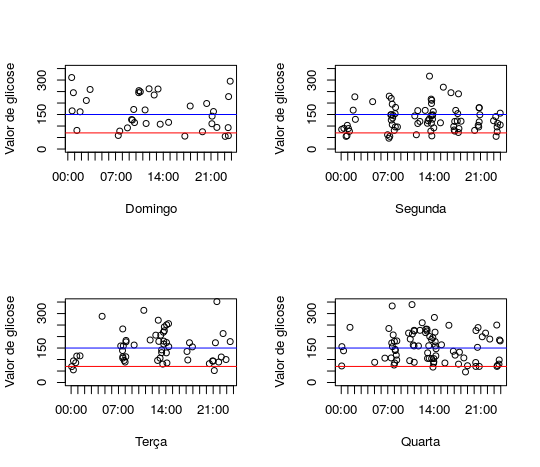
\includegraphics[scale=0.8]{/home/tiago/Tese/Tese/Databases/CSV/Data/ImagensTese/Utilizador2/Days.png}
\caption{Glicemia por horas do utilizador 2}
\end{figure}

\begin{figure}[H]
\centering
\includegraphics[scale=0.8]{/home/tiago/Tese/Tese/Databases/CSV/Data/ImagensTese/Utilizador2/Dias2.png}
\caption{Glicemia por horas do utilizador 2}
\end{figure}

Observando as figuras verifica-se que o utilizador apresenta hiperglicemias todos os dias, maioritariamente durante a tarde. Ao Domingo apresenta menos hiperglicemias porque também tem menos registos. No resto dos dias apresenta uma distribuição semelhante entre valores normais e valores acima do limite de hiperglicemia, isto é, há mais ou menos quantidade de valores normais e valores demasiado altos. Contudo, ao Sábado o número de hiperglicemias é bastante maior em relação ao número de valores no intervalo normal.



\textbf{Utilizador 3}

\begin{figure}[H]
\centering
\includegraphics[scale=0.8]{/home/tiago/Tese/Tese/Databases/CSV/Data/ImagensTese/Utilizador3/Dias.png}
\caption{Glicemia por horas do utilizador 3}
\end{figure}

\begin{figure}[H]
\centering
\includegraphics[scale=0.8]{/home/tiago/Tese/Tese/Databases/CSV/Data/ImagensTese/Utilizador3/Dias2.png}
\caption{Glicemia por horas do utilizador 3}
\end{figure}


Neste utilizador é possível ver um padrão: tem tendência para ter hiperglicemias de manhã e ao fim da tarde ou início da noite. Uma vez mais, a causa pode estar relacionado com o trabalho, por exemplo, que pode ser mais desgastante à tarde, daí fazer com que os valores não subam tanto. Esta teoria seria ainda suportada pelo gráfico de Sábado, que mostra algumas hiperglicemias também a meio da tarde, o que faria sentido se de facto a causa dos valores durante a semana fosse o trabalho. 

\textbf{Utilizador 4}

\begin{figure}[H]
\centering
\includegraphics[scale=0.8]{/home/tiago/Tese/Tese/Databases/CSV/Data/ImagensTese/Utilizador4/Dias.png}
\caption{Glicemia por horas do utilizador 4}
\end{figure}

\begin{figure}[H]
\centering
\includegraphics[scale=0.8]{/home/tiago/Tese/Tese/Databases/CSV/Data/ImagensTese/Utilizador4/Dias2.png}
\caption{Glicemia por horas do utilizador 4}
\end{figure}


Observando as figuras em cima, é possível observar que em todos os dias ocorrem hiperglicemias mas há três dias que se destacam: Domingo, Segunda e Terça, pois têm mais hiperglicemias em comparação com valores normais que o resto dos dias. Verifica-se também que os valores mais altos ocorrem de manhã ou ao início da noite, sendo que apenas em dois dias há mais que uma hiperglicemia a meio da tarde, o que pode significar que o utilizador possa fazer algo de diferente nestes dois dias, embora sem qualquer tipo de certeza. 
Em vários dias da semana notam-se alguns valores muito próximos ou até abaixo do limite de hipoglicemia sendo notórios dois períodos em que eles são mais frequentes: durante a madrugada e perto da hora de almoço. Isto pode significar que o utilizador come nada antes de ir dormir, para o primeiro caso, e para o segundo caso pode significar que o utilizador não come nada entre o pequeno-almoço e o almoço, e que talvez devesse comer alguma coisa. 


\textbf{Utilizador 5}

\begin{figure}[H]
\centering
\includegraphics[scale=0.8]{/home/tiago/Tese/Tese/Databases/CSV/Data/ImagensTese/Utilizador5/Dias.png}
\caption{Glicemia por horas do utilizador 5}
\end{figure}

Para este utilizador mostramos apenas gráficos referentes a três dias já que os outros não têm registos suficientes